% Hier wird der theoretische Teil vorgenommen. 

\chapter{Stand der Technik}


\section{Ähnlichkeitsmaße}

Im Folgenden sollen Ähnlichkeitsmaße zwischen Mengen, insbesondere 
solche, die als Kostenfunktion bzw. Bewertungsmetrik für einen binären 
Klassifikator verwendet werden können, untersucht werden. Hierzu wird zunächst Cross-Entropy betrachtet,
gefolgt von dem Dice- bzw. F-Maß. Weiter werden \ac{IoU} und das darauf aufbauende Quality-Maß betrachtet.

\subsection{\acf{BCE}}

Die \textit{Cross-Entropy} (bzw. dt. \textit{Kreuzentropie}) ist ein Maß des Unterschieds zweier
Wahrscheinlichkeitsdistributionen. Im Spezialfall einer binären Wahrscheinlichkeitsvariable 
kann die Cross-Entropy zur \textit{\acf{BCE}} spezialisiert werden, um auf ein binäres 
Klassifikationsproblem angewandt zu werden. 
\autoref{eq:bce} zeigt die Kalkulation von \ac{BCE}, wobei $p \in [0;1]$ die Prediction 
eines binären Klassifikators und $y \in {0,1}$ der Wert des Labels darstellen.
\begin{align}
	\label{eq:bce} BCE = -[p \cdot \log(y) + (1-p) \cdot \log(1-y) ]
\end{align} 
Um über $n$ Prediction-Label-Paare $(p_i; y_i)$ den \ac{BCE} zu berechnen, wird das arithmetische Mittel nach
\autoref{eq:bce-mean} gebildet \cite[S.~82]{Cybenko.1999}[S.~57--59]{Murphy.2012}.
\begin{align}
	\label{eq:bce-mean} BCE = -\frac{1}{n}\sum_{i = 1}^{n}[p_i \cdot \log(y_i) + (1-p_i) \cdot \log(1-y_i) ]
\end{align}

Im Sinne einer differenzierbaren Kostenfunktion im Kontext von \ac{ML} sind \ac{BCE},
\textit{negative Log-Likelihood} und \textit{Logistic-Regression} synonym \cite[S.~249]{Murphy.2012}. 

Aus \autoref{eq:bce-mean} geht hervor, warum \ac{BCE} gut geeignet für Klassifikationsprobleme ist.
Im Gegensatz zum mittleren absoluten Fehler, bei dem ein Fehler linear eingeht, und zum mittleren quadratischen Fehler,
bei dem ein Fehler quadratisch eingeht, geht ein Fehler bei \ac{BCE} exponentiell ein. 
Ein größerer Fehler wiegt also exponentiell stärker als ein kleinerer Fehler. 
Hierdurch werden die Fehler pro Datenpunkt und Klasse sehr klein, 
wodurch gute Performance und gute Generalisierung bei \ac{ML}-Modellen erreicht werden können. \\

Bei stark ungleichmäßiger Klassenverteilung kann es jedoch dazu kommen, 
dass die unterrepräsentierte Klasse kaum noch geschätzt wird, 
da der Fehler einer falsch geschätzten überrepräsentierten Klasse zu stark bestraft wird.
Dadurch lernt der Algorithmus, die unterrepräsentierte Klasse kaum zu schätzen.
Eine Abhilfe dagegen schafft eine Gewichtung der unterschiedlichen Klassen \cite[S.~4]{Ronneberger.18052015}.

\subsection{Dice- und F-Maß}

Das \textit{Dice-}, oder auch \textit{Sorensen-Dice-}Maß $D$ wurde 1945 bzw. 1948 erstmals vorgestellt und genutzt, um die Ähnlichkeit zweier botanischer Stichproben zu ermitteln. Verallgemeinert auf diskrete Mengen $X$, $Y$ kann deren Ähnlichkeit nach Dice $D$ beschrieben werden durch \autoref{eq:dice-coeff}. Es gilt $D \in [0; 1]$ \cites[S.~33]{Srenson.1948}[S.~297]{Dice.1945}. 
\begin{align}
	\label{eq:dice-coeff} D = \frac{2 \cdot | X \cap Y |}{2 \cdot | X \cap Y | + |Y \setminus X| + |X \setminus Y|} 
	=\frac{2 \cdot | X \cap Y |}{|X| + |Y|}
\end{align} 

Angewandt auf boolesche Mengen und binäre Klassifikatoren ist das Dice-Maß gleich dem $F_1$-Maß, das ein Maß für die Qualität eines statistischen Tests darstellt. Dafür sei $X$ nun die Menge der positiven Elemente und $Y$ die Menge der als positiv eingestuften Elemente. Dann ist die \textit{Genauigkeit} oder auch \textit{Precision} gegeben durch
\begin{align}
	\label{eq:precision} precision = \frac{|X \cap Y|}{|Y|}
\end{align}
der Anteil der richtig eingestuften Elemente an allen positiv eingestuften Elementen und die \textit{Trefferquote} oder auch \textit{Recall} gegeben durch
\begin{align}
	\label{eq:recall} recall = \frac{|X \cap Y|}{|X|}
\end{align}
der Anteil der richtig eingestuften Elemente an allen positiven Elementen. \\
Das F-Maß, bzw. genauer das $F_1$-Maß, ist dann gegeben durch das harmonische Mittel aus Precision und Recall, wobei $tp$ die Anzahl von wahr-positiven, $fp$ die Anzahl von falsch-positiven und $fn$ die Anzahl von falsch-negativen Elementen ist \cite{YutakaSasaki.2007}:
\begin{align}
	\label{eq:f1} F_{1} = \frac{2\cdot precision \cdot recall}{precision + recall} = \frac{2\cdot tp}{2 \cdot tp + fp + fn}
\end{align}
Precision und Recall können mit einem Faktor $\alpha$ unterschiedlich zueinander gewichtet werden, um mit $F_{\alpha}$ unterschiedliche Aspekte zu fokussieren. 

Das Dice-, bzw. $F_{\alpha}$-Maß kann leicht für eine differenzierbare Kostenfunktion genutzt werden mit Dice-Loss $D_{L}(X, Y) = 1 - D(X,Y)$, bzw. $F_{\alpha}$-Loss $F_{\alpha L}(X,Y) = 1 - F_{\alpha}(X,Y)$. 


\subsection{\acf{IoU}}

Die \textit{\acf{IoU}-} bzw. \textit{Jaccard-Ähnlichkeitsmetrik} ist ein weit verbreitetes Maß zur Bestimmung der Ähnlichkeit zwei diskreter Mengen. Hierzu seien $X$ und $Y$ diskrete Mengen. Dann ist die $IoU$ gegeben durch 
\begin{align}
	\label{eq:iou} IoU = \frac{|X\cap Y|}{|X \cup Y|} = \frac{| X \cap Y |}{| X \cap Y | + |Y \setminus X| + |X \setminus Y|}~.
\end{align} 
Für ein binäres Klassifikationsproblem lässt sich die $IoU$ ausdrücken durch 
\begin{align}
	\label{eq:iou-binary} IoU = \frac{tp}{tp + fp + fn}~,
\end{align}
wobei $tp$, $fp$, $fn$ wie in \autoref{eq:f1} \cite{Fletcher.2018}. 

Auffällig ist die Ähnlichkeit zum Dice- bzw. $F_{1}$-Maß. Es ist allerdings anzumerken, dass bei Dice/$F_1$ die $tp$, also die wahr-positiven, stärker gewichtet werden, als bei der \ac{IoU}. Die augenscheinliche Ähnlichkeit lässt sich durch die Beziehungen
\begin{align}
	\label{eq:dice-iou} IoU = \frac{D}{2 - D} \\
	D = \frac{2 \cdot IoU}{1 + IoU}
\end{align}
beschreiben.
Im Gegensatz zur \ac{IoU} wird beim Dice-Maß eine höhere Gewichtung auf die wahr-positiven Elemente 
gelegt.

\subsection{Quality}

Bei der \textit{Quality} handelt es sich um eine gepufferte Form des \ac{IoU},
die toleranter bezüglich der Lokalität der Elemente der verglichenen Mengen, oder konkreter,
der Pixel einer semantischen Segmentierung, ist, 
wobei für dieselbe Eingabe $Quality \geq IoU$; $Quality \in [0;1]$ gilt, abhängig von der Puffergröße. 
Die Quality wird analog zur \ac{IoU} über eine gepufferte Precision - die \textit{Correctness} - 
und über einen gepufferten Recall - die \textit{Completeness} - berechnet. Insbesondere werden einige Elemente, 
die zuvor als $fp$ und $fn$ eingeordnet wurden, hiermit zu $tp$ konvertiert. \\
Die Quality soll einige Probleme der \ac{IoU} beheben, um ein Ähnlichkeitsmaß darzustellen, 
was näher an der praktischen und vom Menschen wahrgenommen Leistung eines \ac{ML}-Modells zur semantischen Segmentierung liegt.
So soll relativiert werden, dass vor allem im Randbereich einer Segmentierung einzelne abweichende Pixel
nicht als falsch anerkannt werden, sodass die Segmentierung im Großen und Ganzen als richtig anerkannt wird \cite{ChristianWiedemann.1998}. 


\section{Architekturkomponente}

Im Folgenden werden verschiedene Architekturkomponenten diskutiert, die im \ac{ML} allgemein 
bzw. bei semantischer Segmentierung im Speziellen verwendet werden. Hierzu werden zunächst Dropout-Layer 
und Batch-Normalization-Layer begutachtet und dann die U-Net-Architektur zur semantischen Segmentierung vorgestellt. 

\subsection{Dropout}

\textit{Dropout} ist eine ressourcenschonende Regularisierungstechnik für \ac{ML}-Modelle. 
Hierbei werden einzelne Neuronen mit einer Wahrscheinlichkeit von \textit{Rate} $r$ während des Trainings 
deaktiviert, also deren Output auf $0$ gesetzt.\\ 
Da bei der Inferenz Dropout dazu führen kann, 
dass wichtige Features ignoriert werden, ist Dropout während der Inferenz unerwünscht. Ohne Dropout während der 
Inferenz sind allerdings alle Gewichte aktiv, was zu einer höheren Summe der Gewichte während der Inferenz, 
als während des Trainings führt. Deswegen müssen die Gewichte für die Inferenz nach unten skaliert werden. 
Alternativ können während des Trainings alle Gewichte nach oben skaliert werden, die nicht deaktiviert wurden. 
Somit muss für die Inferenz keine Anpassung vorgenommen werden. Nach jedem Trainings-Batch werden die aktivierten 
Neuronen dann um Faktor $\frac{1}{1-r}$ skaliert werden \cites[S.~255--258]{Goodfellow.2016}{NitishSrivastava.2014}.

Es hat sich gezeigt, dass Dropout eine effektivere Regularisierungstechnik zur Minderung von Overfitting ist, 
als andere ressourcenschonende Techniken, wie \textit{Weight-Decay}, \textit{Filter-Norm-Constraints} oder 
\textit{Sparse-Activity-Regularization}, wobei Dropout mit diesen kombiniert werden kann, für noch bessere 
Regularisierung \cites[S.~265]{Goodfellow.2016}.

\subsection{Batch-Normalization}

\textit{Batch-Normalization} normalisiert und standardisiert den Output von Neuronen auf Basis des Mittelwerts 
und der Streuung einer Batch während des Trainings. Für die Inferenz werden Durchschnittswerte 
des Mittelwerts und der Streuung der Batches des Trainingsdatensatzes herangezogen und angewandt. \\
Batch-Normalization führt zu einer schnelleren Konvergenz im Training, 
sodass die Anzahl an benötigten Epochen in manchen Fällen halbiert werden können. Des Weiteren führt 
Batch-Normalization zu einer gewissen Regularisierung, da es die Kostenfunktion zu einem gewissen Grad glättet 
\cites[S.~317--320]{Goodfellow.2016}{Ioffe.11022015}.
Besonders gut funktioniert Batch-Normalization für \acp{CNN} und Netzwerke mit Sigmoid-Aktivierungsfunktion
\cites[S.~425]{Goodfellow.2016}.

\subsection{U-Net}

Die \textit{U-Net-Architektur} beschreibt eine \textit{Fully-Convolutional-Network-Architektur}, die erstmals in Freiburg 2015 vorgestellt wurde 
und herausragende Ergebnisse für verschiedene Benchmarks, insbesondere zur semantischen Segmentierung kleiner Datensätze, liefert. \\
Aus \autoref{fig:u-net-architecture} geht die namensgebende Architektur der U-Net hervor. Die folgenden Besonderheiten 
führen zu der sehr guten Performanz des Netzes bei semantischer Segmentierung \cite{Ronneberger.18052015}:
\begin{itemize}
	\item Das Netz besteht aus einem kontrahierenden Encoder-Teil (linke Hälfte) und einem expandierenden und symmetrisch aufgebauten
	Decoder-Teil (rechte Hälfte). Der Encoder erzeugt feinere \textit{Feature-Maps} mit zunehmender Netztiefe, 
	während der Decoder diese wieder extrapoliert, was zu einer besseren Lokalisierung führt. 
	\item Zwischen den jeweiligen symmetrischen Encoder- bzw. Decoder-Blöcken befinden sich \textit{Skip-Connections}\footnote{\textit{copy and crop} in der Abbildung.}.
	Zusammen mit dem vorherigen Punkt erhöht dies weiter die Lokalisierung und Performanz, da der jeweilige Decoder-Block feinere Features von der \textit{Up-Convolution}\footnote{implementiert als \textit{Transposed Convolutions}.},
	wie auch den größeren Kontext von früheren Blocks mittels Skip-Connection erhält. 
	\item Zur Mitte des Netzes hin erhöht sich die Anzahl der Convolution-Filter und damit die Anzahl der \textit{Channel}, 
	während sich die Dimensionen der einzelnen Feature-Maps durch das \textit{Downsampling} verringert. 
	Hierbei ist anzumerken, dass bei der Implementation kein \textit{Padding} für die Convolutions verwendet wurde,
	wodurch sich die Dimensionen der Feature-Maps nach jeder Convolution verringert. 
	Hieraus folgt ein Zuschneiden für die Skip-Connections. 
\end{itemize}

\begin{figure}
	\centering
	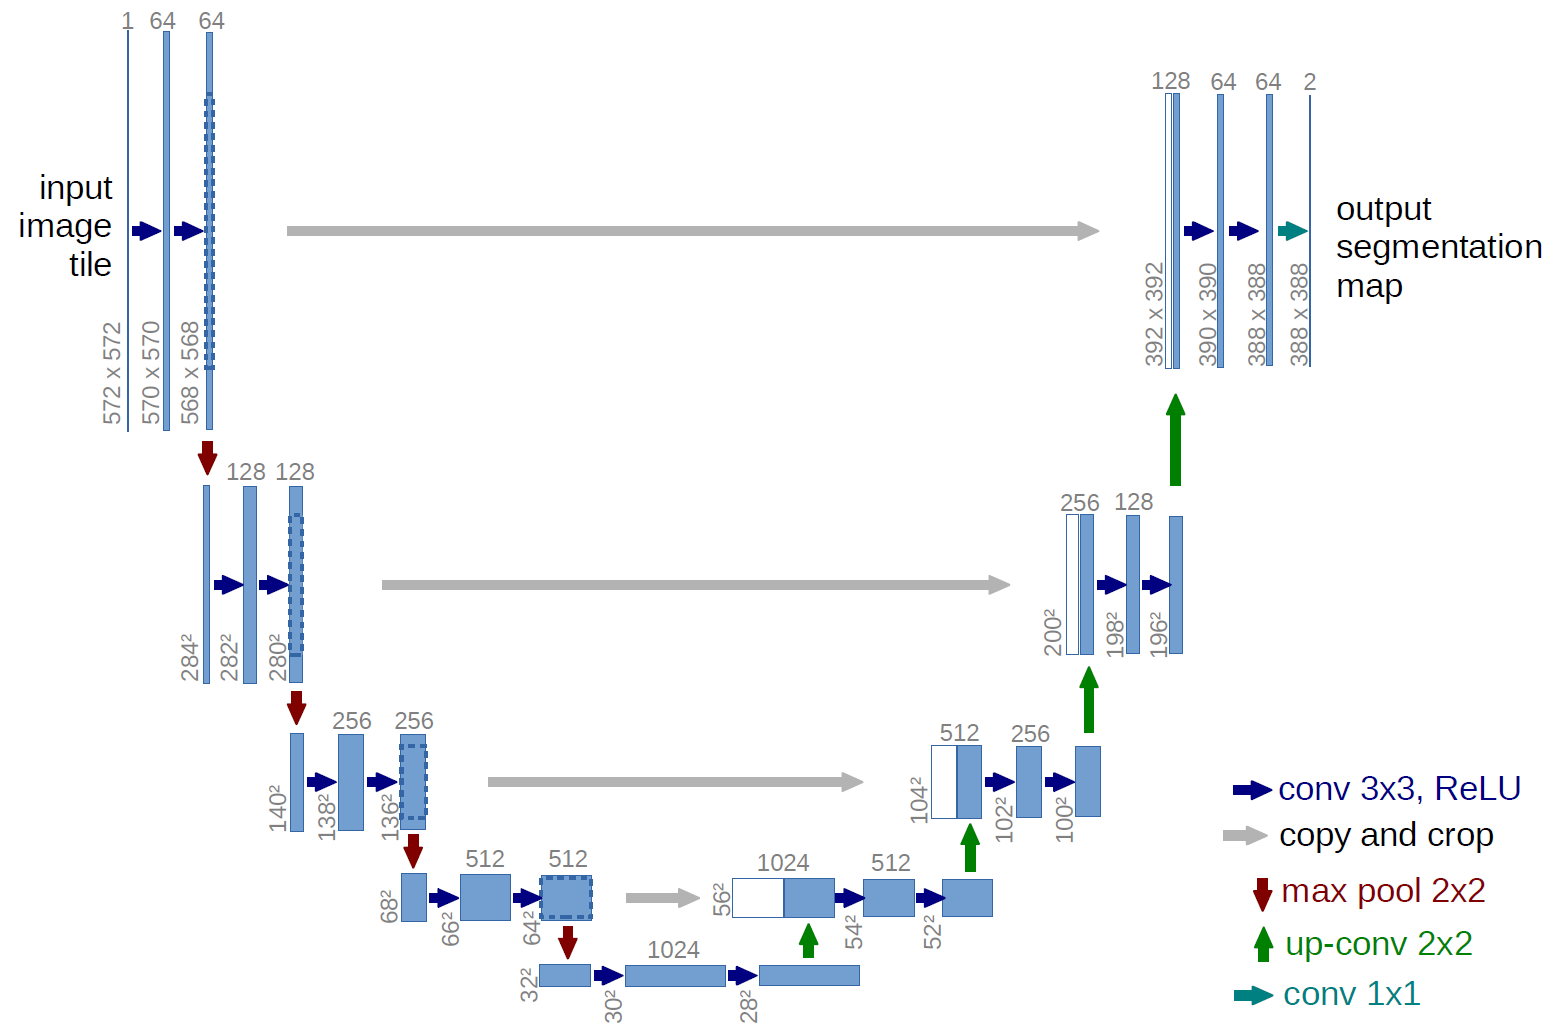
\includegraphics[width=0.8\textwidth]{Bilder/u-net-architecture.png} 
	\caption{Ursprüngliche U-Net-Architektur \cite{Ronneberger.18052015}.}
	\label{fig:u-net-architecture}
\end{figure} 


\section{Transfer-Learning mit U-Net}

\textit{Transfer-Learning} beschreibt das Übertragen von trainierten Gewichten eines \ac{ML}-Modells auf ein anderes, 
bestenfalls ähnliches Problem und Modell. Das Modell wird dann via \textit{Fine-Tuning} verfeinert mit dem neuen Datensatz und unterschiedlichen Trainingsmethoden.
Häufig wird dafür ein Teil des Modells eingefroren, sodass sich die eingefrorenen Gewichte nicht verändern können. Dies verhindert, 
dass die bereits vortrainierten Gewichte durch die erste Trainings-Batch zerstört werden. Eine weitere Möglichkeit ist,
mit einer sehr geringen Lernrate das gesamte Modell zu trainieren. Oft werden beide Ansätze auch verbunden.

Der Vorteil von Transfer-Learning liegt darin, dass das Training deutlich kürzer dauert, 
weil direkt mit einer höheren Genauigkeit eingestiegen wird, mit kleineren Datensätze bessere Ergebnisse erzielt werden können
 und auch insgesamt eine höhere Genauigkeit 
am Ende des Trainings erreicht wird, als bei herkömmlichen Training. Diese Effekte sind verstärkt, 
abhängig davon, wie ähnlich der Datensatz des Pre-Trainings und des eigentlichen Trainings sind \cite{Ruder.3212017}. \\
Insbesondere bei Computer-Vision ist Transfer-Learning effektiv, da bei Bildern high-level Features wie Clustering 
ähnlichfarbener Pixel oder Kantenerkennung oftmals sehr ähnlich zwischen unterschiedlichen Datensätzen ausfallen 
und damit schon vorhanden sind \cite{Ruder.3212017}. 

Für Transfer-Learning mit U-Nets gibt es verschiedene Strategien: Backbone-Netze als Encoder, 
partielles Einfrieren verschiedener Netzbereiche und direktes Trainieren mit geringer Learning-Rate.
Der Stand der Wissenschaft diesbezüglich wird im Folgenden vorgestellt. 

\subsection{Training mit Backbones}

Im Kontext von Transfer-Learning bei U-Nets bezeichnet ein \textit{Backbone} ein etabliertes vortrainiertes \ac{CNN}, 
welches, leicht modifiziert, als Encoder für das U-Net verwendet wird. Hierbei wird der Decoder-Teil des U-Net 
symmetrisch dem Encoder nachempfunden und an passenden Stellen Skip-Verbindungen zwischen En- und Decoder eingebaut. \\
Hierdurch kann eine geeignete \ac{CNN}-Architektur für das spezifische Problem ausgewählt werden. Des Weiteren sind diese 
Modelle auf sehr großen Datensätzen, wie \textit{ImageNet}, vortrainiert öffentlich zugänglich. 

Bei der semantischen Segmentierung von medizinischen Lungen-Ultraschall-Bildern, wurden die besten Ergebnisse von einem Dice-Maß-Standpunkt aus, 
mit einem U-Net mit auf ImageNet trainierten \textit{VGG16}-Backbone erzielt. Das Vergleichsnetz, welches zuerst auf dem \textit{Salien Object}
Datensatz vortrainiert wurde, erzielte schlechtere Ergebnisse von dem Dice-Maß her, wobei allerdings das VGG16-U-Net kleine falsch-positive 
Regionen erkannte, die weit Außerhalb der Ground-Truth lagen. Die falsch-positiven beim Vergleichsnetz, lagen direkt an der Ground-Truth, 
dies lässt auf eine sensitivere Kantenerkennung beim VGG16-U-Net schließen, die manchmal aber auch übersensitiv war \cite{Cheng.05.10.2021}. 

Für das Training des VGG16-U-Nets wurde der Encoder-Teil eingefroren und somit nur der Decoder trainiert. 

\subsection{Partielles einfrieren und Training mit geringer Lernrate}

Im oben beschriebenen Problem zur semantischen Segmentierung wurde das vortrainierte Vergleichsnetz auf zwei Weisen fein-trainiert:
\begin{enumerate}
	\item Ohne Einfrieren mit einer Lernrate von $10^{-5}$
	\item und mit Einfrieren des mittleren Blocks, welcher ungefähr $14\cdot 10^6$ der insgesamt $31 \cdot 10^6$ Parameter enthielt. 
\end{enumerate}
Die 5-fache Kreuzvalidierung ergab sowohl für den besten Lauf, als auch für den durchschnittlichen Lauf, ein besseres Dice-Maß 
für das Training aller Parameter. In keinem der Fälle gab es, anders als beim VGG16-U-Net, segmentierte Regionen ohne Zusammenhang mit der Ground-Truth \cite{Cheng.05.10.2021}. 

In einem weiteren Paper wurde untersucht, welche Layer eines U-Net am besten eingefroren werden sollten, für das Fine-Tuning von medizinischen Bildern - 
zum einen von Lungen-Ultraschall-Bildern und zum anderen von Brust-Röntgen-Aufnahmen. 
Hier wurde wieder mit dem \textit{Salien Objetcs} Datensatz vortrainiert. Dann wurden für beide Anwendungsfälle folgende Tests durchgeführt: 
\begin{enumerate}
	\item Einfrieren der linken Hälfte (Encoder) des Netzes,
	\item Einfrieren der rechten Hälfte (Decoder) des Netzes,
	\item gesamtes Netz, bis auf den ersten Block eingefroren und dann nach jeweils fünf Epochen sukkzessive weitere Blöcke freigeben und
	\item dasselbe allerdings von hinten nach vorne.
\end{enumerate}
Für die Röntgenaufnahmen gab es keine Unterschiede, wobei der Dice-Score hier allerdings auch bei $0.98$ lag. 
Für die Ultraschallbilder lieferte Methode (1) die schlechtesten Ergebnisse (Dice: $0.72$), gefolgt von Methode (2) (Dice: $0.80$) 
und gleichermaßen (3) und (4) (Dice: $0.82$), wobei (3) deutlich schneller konvergierte \cite{Amiri.19.02.2020}.



\section{Graphentheorie}

Dieser Abschnitt wird grundlegende graphentheoretische Begriffe definieren, die Darstellung in Computersystemen diskutieren, sowie einige einfache Algorithmen anführen, die für die weitere Arbeit relevant sind.

\subsection{Definitionen}


\textbf{Teilgraph} \\
Sei $G = (V, E)$ ein Graph. $T = (V', E') \subseteq G$ mit $V' \subseteq V$ und $E' \subseteq \{\{x,y\} \in E \mid x, y \in V'\}$ heißt \textit{Teilgraph} von $G$ ~\cite[S.~4]{Diestel.2016}.  


\textbf{Eingangs- und Ausgangsgrad im Digraph} \\
Sei $G = (V, E)$ ein Digraph und $v \in V$ ein Knoten in $G$, dann heißt $d^-_G(v) = | \{(x, y) \in E \mid y = v\} |$ der \textit{Eingangsgrad} von $v$ und $d^+_G(v) = | \{(x, y) \in E \mid x = v\} |$ der \textit{Ausgangsgrad} von $v$. Im klaren Kontext kann die Indizierung mit dem Graphen weggelassen werden. Knoten $v$ mit $d^-(v) = 0$ heißen  \textit{Quellen} und Knoten $v$ mit $d^+(v) = 0$ heißen  \textit{Senken} ~\cite[S.~460]{Satyanarayana.2014}.

\textbf{Pfade} \\ 
Ein \textit{Pfad} ist ein nicht-leerer, gerichteter Graph $P = (V, E)$ der Form $V = \{x_0, x_1, ..., x_k\};~E=\{(x_0,x_1), (x_1, x_2), ..., (x_{k-1}, x_k)\}$ wobei alle $x_i$ paarweise verschieden sind. Die Knoten $x_0$ und $x_k$ heißen \textit{Endknoten} (bzw. \textit{Start-} und \textit{Endknoten} im Digraph) und sind \textit{verbunden} durch $P$ ~\cite[S.~6]{Diestel.2016}. Pfade lassen sich auch als Folge ihrer aufeinander folgenden Knoten schreiben: $P = x_0x_1...x_k$ ~\cite[S.~7]{Diestel.2016}~\cite[S.~475]{Sedgewick.1992}. 


\textbf{Zyklen} \\
Sei $P = x_0...x_{k-1}$ ein Pfad und $k \geq 3$, dann ist der Graph $C := P + x_{k-1}x_0 = x_0...x_{k-1}x_0$ ein \textit{Zyklus} ~\cite[S.~8]{Diestel.2016}~\cite[S.~475]{Sedgewick.1992}.


\textbf{Transitive Hülle eines Knotens} \\
Sei $G = (V, E)$ ein Graph und $v \in V$ ein Knoten in $G$. Im Kontext
 dieser Arbeit sei die \textit{transitive Hülle eines Knotens} $v$ definiert
  als der Teilgraph $v^*_G := (V_v, E_v) \subseteq G$ 
  mit $V_v = \{x \in V \mid \exists P \subseteq G: P=x...v\}$ 
  und $E_v = \{ (x,y) \in E \mid x,y \in V_v \}$. 
  Also der Teilgraph in $G$, der alle Knoten und dazugehörigen Kanten enthält, von denen $v$ erreichbar ist. Es handelt sich bei dieser Definition also um einen \enquote{umgekehrten Erreichbarkeits-Teilgraph} ~\cite[S.~41--42]{Sandner.01.09.1998}.



\subsection{Tiefensuche (DFS)}

\autoref{code:dfs} zeigt eine Implementation der Funktion zur rekursiven Tiefensuche in C++ mit Adjazenzlisten als Graphrepräsentation. Hierbei ist \code{adj} ein Feld mit den (Adjazenz-)Listen und \code{visited} ein Array, welches jedem Knoten die Markierung ob er schon besucht wurde zuweist.

\lstinputlisting[
	label=code:dfs,    % Label; genutzt für Referenzen auf dieses Code-Beispiel
	caption=Rekursive Implementation der Tiefensuche mit Adjazenzlisten in C++. (In Anlehnung an \cite{GeeksforGeeks.2012}.),
	captionpos=b,               % Position, an der die Caption angezeigt wird t(op) oder b(ottom)
	style=EigenerCppStyle,   % Eigener Style der vor dem Dokument festgelegt wurde
	firstline=1,                % Zeilennummer im Dokument welche als erste angezeigt wird
	lastline=8                 % Letzte Zeile welche ins LaTeX Dokument übernommen wird
]{Quellcode/dfs.cpp}


\section{Submodelle} \label{sec:submodelle}

Die Submodelle werden durch die \ac{ProdDeco} aus dem (Haupt-)Modell des Szenarios erstellt. Dabei wird für \ac{SNP} und \ac{SOP} gleichermaßen verfahren. 

\subsection{Elementtypen} \label{sec:elements}
Das Modell eines Szenarios beinhaltet Elemente mit verschiedenen Elementtypen, wovon die wichtigsten im Folgenden vereinfacht vorgestellt werden:

\begin{itemize}
\item \textit{Quota Arrangement} - Ein vordefiniertes Kontingent an Materialbezug bzw. Materialverteilung, welches während des Optimierungslaufs strikt eingehalten werden muss \cite{.20220812c}. \\ Ein Beispiel wäre hierfür: Es werden 100 Stück von Produkt P1 an Lokation L1 benötigt. Es bestehen folgende Quota Arrangements: \begin{itemize}
\item Genau 40\% des Bedarfs müssen über einen Transport von Lokation L2 gedeckt werden.
\item Mindestens 10\% müssen über einen Transport von Lokation L3 gedeckt werden.
\item Genau 20\% müssen von einer Produktion in L1 gedeckt werden.
\end{itemize} 
\item \textit{Ressource} - Ein lokations-gebundenes Asset mit begrenzter Kapazität, welches eine bestimmte Funktion in der Supply Chain erfüllt. Die Ressource gehört zu genau einer Lokation, aber ihre Kapazität kann auf mehrere Produkte aufgeteilt werden. Beispiele: Eine Maschine, eine Person, ein Lager oder ein Transportmittel \cite{.20220812b}.
\end{itemize}

\section{Ähnlichkeitsmaße zwischen Graphen in der Literatur} \label{sec:sim_lit}

Im Folgenden wird eine Auswahl an Ähnlichkeitsmaßen zwischen Graphen aus der Literatur vorgestellt.

\subsubsection{Azyklischer Graph Edit Distance} \label{sec:sim_edit_dist}

Die \textit{Azyklischer Graph Edit Distance} beschreibt die minimale Anzahl an elementaren Veränderungen (Einfügen, Löschen, Umbenennen von Knoten), die durchgeführt werden müssen, um aus einem azyklischen (ungerichteten) Graph einen anderen zu machen \cite{Zhang.1989}. Hierbei wird allerdings rein die Ähnlichkeit der Struktur ermittelt.

\subsubsection{Similarity Flooding} \label{sec:sim_flooding}

Beim \textit{Similarity Flooding} wird die initiale Ähnlichkeit zweier Elemente aus zwei zu vergleichenden Graphen berechnet und diese Ähnlichkeit dann per Fixpunktiteration an benachbarte Knoten propagiert \cite{S.Melnik.2002}. Es läuft also unter der Annahme, dass aus dem Finden zweier ähnlicher Elemente eine Ähnlichkeit für die Nachbarelemente folgt. 

\subsubsection{Similarity of Weighted Directed Acyclic Graphs} \label{sec:sim_dag}

Sei $G = (V, E)$ ein \ac{DAG}. \textit{Similarity of Weighted Directed Acyclic Graphs} beschreibt einen Algorithmus zur effizienten Bestimmung der Ähnlichkeit von weighted \acp{DAG} \cite{Jin.2004}.
 
\begin{figure}
	\centering
	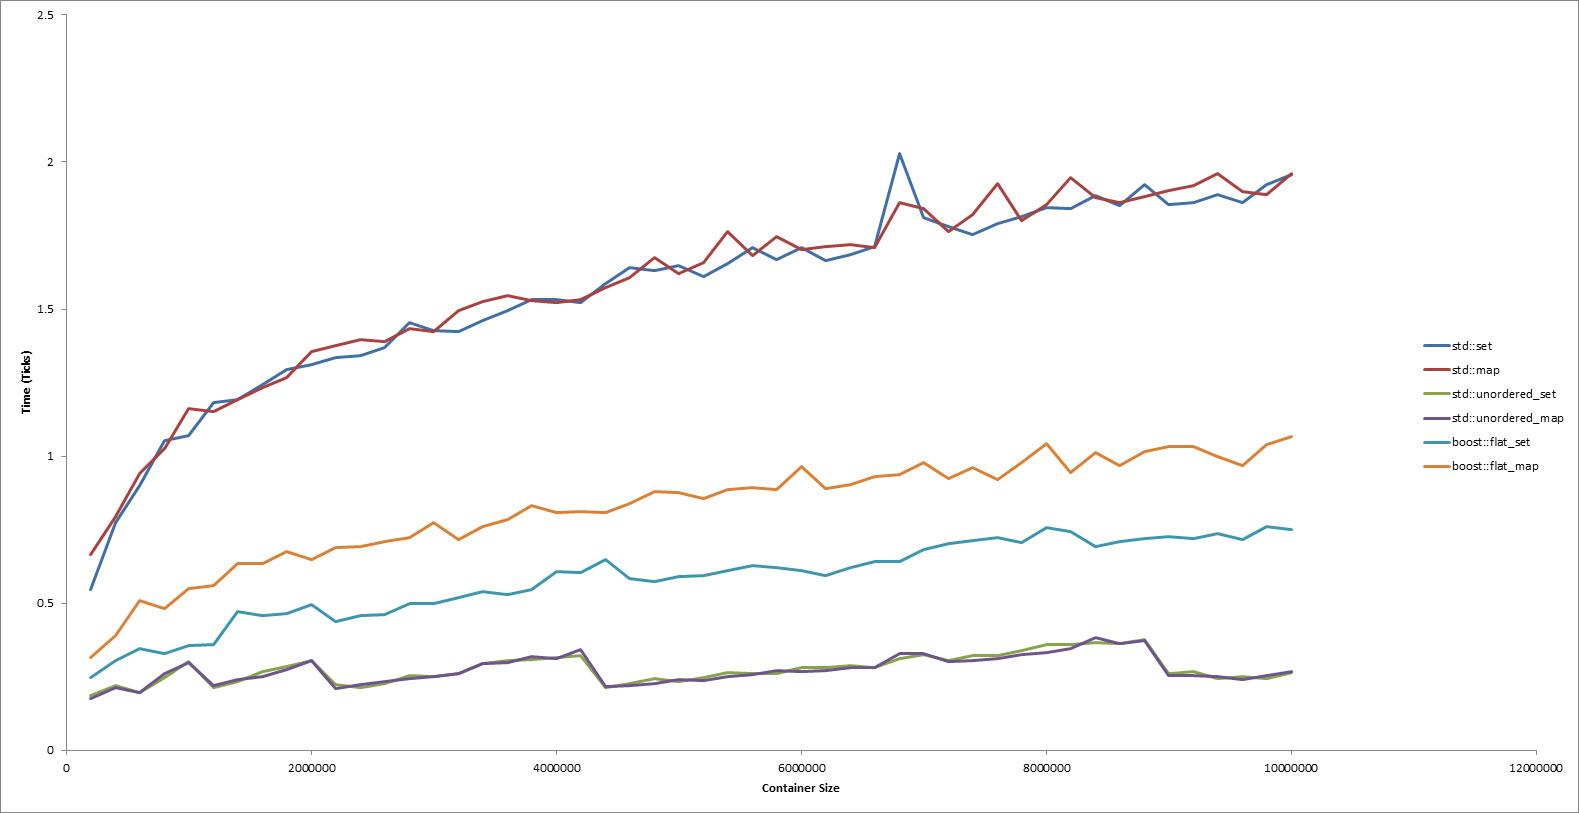
\includegraphics[width=\textwidth]{Bilder/GCC_timings_10M.jpg} 
	\caption{Lookup-Performanceunterschiede zwischen Map (rot), Set (blau), Flat\_Map (gelb), Flat\_Set (hellblau), Hash-Map (violett), Hash-Set (grün). Abszisse: Container-Größe 0, 2 Mio., ..., 12 Mio. Ordinate: Time in Ticks.\\ Flat\_X ist herbei ein sortierter Vektor \cite{.20220811}.\\ (Abb. entnommen aus \cite{.20220819b}.)}
	\label{fig:container_perf}
\end{figure} 
